\chapter{Theory}
\label{chapter:Theory}
%
% By training, the author would describe himself as an Engineer.  Nevertheless,
% the following excursion into "Theory" reflects his search for deeper understanding
% of the theory which he applies.  The following commentary is meant to offer the reader
% insight into the authors understanding, and manner of dealing with relative complexity,
% and not to revolutionize the fields of Mathematics or Computer Science.  The
% experience of completing this work and composing this document has been a humbling one.

\section{Problem Setting}
%Boundary Value Problems
In the scope of this work, we consider the elliptic boundary value problem of
the Poisson's equation
\eqref{eq:poisson} defined as:
  \begin{equation}
    \begin{aligned}
%\forall \text{ domains } \Omega \subset
  %\mathbb{R}^{n}, n \in \mathbb{N} \\ \text{ with }u\colon \Omega \rightarrow \mathbb{R}^{1}\\
  - \bigtriangleup u(x) &= \sigma(x),\quad x \in \Omega,
  \label{eq:poisson}
  \\ u(x) &= f(x),\quad x \in \partial \Omega, \quad (Dirichlet)
\end{aligned}
\end{equation}
where $\Omega \in \mathbb{R}^{n}$ is an open bounded set and $f$ is a function
defined on the boundary $\partial \Omega$.
A special case of the Poisson's equation \eqref{eq:poisson}, is the homogeneous
case, where $\sigma(x) = 0$, called the Laplace's equation
  \begin{equation}
    \begin{aligned}
    \bigtriangleup u(x) &= 0,\quad x \in \Omega,
  \\ u(x) &= f(x),\quad x \in \partial \Omega\text{.}
    \label{eq:laplace}
  \end{aligned}
  \end{equation}
A Dirichlet Boundary Condition is defined as:
\begin{definition}[Dirichlet Boundary Condition]
Given a \Gls{PDE}
defined on a domain $\Omega$, constrained via the definition function values on the
 boundary of the domain $\partial \Omega$, e.g $f(x), \forall  x \in \partial \Omega$
\end{definition}
In this work we be will looking at an approach to numerically solve \eqref{eq:poisson}.
Due to the numerical nature of this task, the solution cannot typically be described symbolically.
Often the solution $u$ is discretized by its function values within $\Omega$, and solved on a grid.
We will be attempting a different approach, but first our goal is to find and exploit the relationship
between \eqref{eq:poisson} and \eqref{eq:laplace} to facilitate a clever numerical solver.
We will therefore examine the possibility to transform a Poisson's equation into
a Laplace's equation, assuming a suitable transformation can be found, in order to
utilize attractive properties thereof.

   Many elliptic \glspl{PDE} can be transformed into harmonic \glspl{PDE},
the properties of which thereby increase the applicability of \gls{RWoS} \cite{Bornemann}.
\newpage
\begin{example}[Transformation of Poisson's equation to Laplace's equation]
Given $u:\Omega \rightarrow \mathbb{R}$ as the solution of
\begin{equation}
  \begin{aligned}
  - \bigtriangleup u(x) &= \sigma(x), \quad x \in \Omega,
  \\ u(x) &= f(x), \quad x \in \partial \Omega,
\end{aligned}
\end{equation}
and $v:\Omega \rightarrow \mathbb{R}$ as the solution of
\begin{equation}
  \bigtriangleup v(x) = 0,\quad x\in\partial\Omega,
\end{equation}
a boundary function $g\in\partial\Omega$ is desired, such that
\begin{equation}
  g(x):=u(x)-v(x), \quad x \in \Omega.
\end{equation}
Therefore we search for a suitable boundary value function $g(x) - w(x), \quad x \in \partial \Omega$.
\begin{equation}
  \begin{aligned}
- \bigtriangleup g(x) &= - \bigtriangleup (u-v)(x) \\
&= - \bigtriangleup u(x) + \bigtriangleup v(x)
\\&= \sigma(x) + 0 = \sigma(x)
\end{aligned}
\end{equation}

This equality also applies on the on $\Omega$, which leads to
\begin{equation}
f(x) = u(x) = g(x) + v(x), \quad x \in \partial \Omega.
\end{equation}
We stipulate
\begin{equation}
\begin{aligned}
  w(x) &= v(x), \quad x \in \partial \Omega\\
  w(x) &= u(x) - g(x) , \quad x \in \partial \Omega,
\end{aligned}
\end{equation}
which defines the transformation boundary condition, and enables the evalutation of
\begin{equation}
  \begin{aligned}
  -\bigtriangleup v(x) &= 0, \quad x \in \Omega\\
  v(x)&=w(x), \quad x \in \partial \Omega
\end{aligned}
\end{equation}

The function $g(x)$  enables us to adjust the boundary value function $w(x)$
so that $v(x)$ fulfills Laplace's equation
\cite{Bornemann}.


\end{example}
An subclass of linear elliptic \Glspl{PDE} is the class of harmonic \Glspl{PDE}, defined as:
\begin{definition}[Harmonic PDEs]
  A \Gls{PDE} whose solution function or function set is harmonic.
\end{definition}
Some special traits harmonic functions will serve as the foundation of the
 following work, and therefore an excursion into their properties and characteristics
is appropriate.

\subsection{Harmonic Functions}\label{sssec:harmonics}
%definition and background from
Harmonic functions are defined by Axler as:
\begin{definition}[Harmonic Function] given $\Omega$ defined as an open, non-empty subset of
  $\mathbb{R}^{n}$, with $n \in \mathbb{N}\setminus \{0,1\}$
  a function $u$ is \textit{harmonic} given it is twice continuously differentiable
  and fulfills $$ \bigtriangleup u \equiv 0$$
\end{definition}

  % discuss properties

  \subsubsection{Mean Value Property}\label{sssec:meanvalue}
  %just describe it don't prove it... don't reinvent the wheel
  For a harmonic $u$ on the closed ball $\bar{B}(a,r)$, centered at $a$ with a radius of $r$,
  it can be proven that $u(a)$ equals the average over $S = \partial \bar{B}(a,r)$\cite{Axler1992,Bornemann}.
\begin{equation}
  \tag{Mean Value Property}
  u(a) = \int_{S} u(a + r\zeta)d\sigma(\zeta)
  \label{eq:mean}
\end{equation}

The following example (see Figure \ref{fig:swingPlot}) is meant to illustrate
the mean value property of harmonic \Glspl{PDE} and will accompany the discussion
of the properties of harmonic functions.

\begin{figure}[ht]
  \centering
  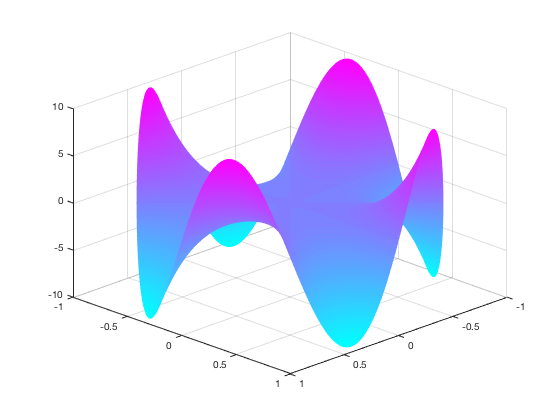
\includegraphics[width=5cm]{styles/swing_function_plot.png}
  \caption{$u(x)$}%{Numerically solved solution}
  \label{fig:swingPlot}
\end{figure}

 The solution of harmonic \glspl{PDE} given the boundary
function $u(\phi)=10\cdot\sin(4\cdot\phi)$ is shown above. The solution function $u(r,\phi)=r^{4}\cdot\sin(4\cdot\phi)$
can be seen on the 2D unit circle $\Omega$.  A known harmonic boundary
condition was defined, and then a solution was solved for analytically by applying the Laplace operator
in polar coordinates to the generalized harmonic function $r^{\alpha}\cdot\sin(4\phi)$,
and solving for $\alpha$.

After integrating over the boundary $\partial \Omega$, it follows that \begin{equation}
u(a) = \int_{S}u(a + r\zeta)d\sigma(\zeta) = \int_{0}^{2\pi} 10\cdot\sin(4\cdot\phi)d\phi = 0,
\label{eq:radinvar}
\end{equation}
which is the solution of $u$ at the center of the 2D unit circle,
namely a =(0,0). As one can deduce from \eqref{eq:radinvar}, for spherical problems, this solution is
radius invariant.  This property is one of the main key stones of \Gls{RWoS}. \label{radiusInvariance}
  \subsubsection{The Maximum Principle}\label{sssec:maximum}
  Following from \ref{sssec:meanvalue} one can make more generalized statements of
  the maximum values of harmonic functions.
  \begin{theorem}
      Let $\Omega$ be connected, and let $u$ be harmonic and real valued function on $\Omega$.
      If $u$ has either a maximum or minimum $\dot{\Omega}$, then $u$ is constant\cite{Sheldon}.
  \end{theorem}

  This property of harmonic functions can be nicely visualized in the solution given
  in figure \ref{fig:swingPlot}. Were one to select any circular
  sub-domain $\omega \subset \Omega$ of the unit circle, one would notice that the maximum value is always
  on the boundary  $\partial \omega$.  Should one claim that the maximum  value be within $\omega$
  the function $u$ would have to be "flat" and therefore constant to fulfill \ref{sssec:meanvalue}.

  \subsubsection{Weighted Mean Value Principle}
  % weights can be compared to probability of hitting a certain boundary based on distribution
  Building on the mean value properties of harmonic functions, one can show that if $u$ is harmonic a
  closed ball $\bar{B}$, then
   \begin{equation}
     u(0) = \int_{S}u(\zeta)d\sigma(\zeta),
     \label{eq:centerval}
    \end{equation}
  then for any $x \in B\text{, }u(x)$ can be expressed as a weighted average of
  $u$ over $S$. Furthermore, there exists a function $P(x,\zeta)$ such that
  \begin{equation}u(x)=\int_{S}P(x,\zeta)u(\zeta)d\sigma(\zeta).\label{eq:weighted_average_integral} \end{equation}
     The function can be shown,
  using the symmetry properties of harmonic functions on a sphere, to be defined as
  \begin{equation}
    \tag{Poisson Kernel for the Ball}
    P(x,\zeta) = \frac{1 - \abs{x}^{2}}{\abs{x- \zeta}^{n}}
    \label{eq:poissonkernel}
  \end{equation}
  in an $n \in \mathbb{N}$ dimensional space \cite{Axler1992}.
\begin{figure}[!htb]%TODO: subfigure
\minipage{0.32\textwidth}
  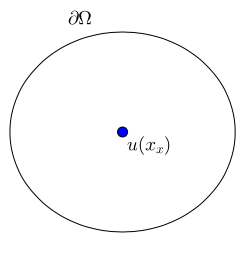
\includegraphics[width=\linewidth]{styles/CircCenter}
  \caption{equation \ref{eq:centerval}}\label{fig:circcenter}
\endminipage\hfill
\minipage{0.32\textwidth}
  \vspace{1.7mm}
  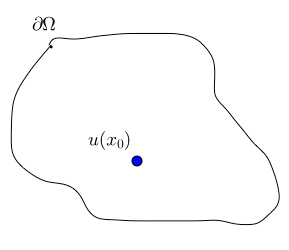
\includegraphics[width=\linewidth]{styles/GeneralOffset}
  \label{fig:generaloffset}
  \caption{equation \ref{eq:weighted_average_integral}}
\endminipage\hfill
\minipage{0.32\textwidth}%
  \vspace{4.5mm}
  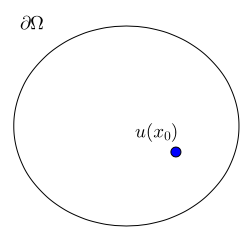
\includegraphics[width=\linewidth]{styles/CircOffset}
  \caption{\ref{eq:poissonkernel}}\label{fig:circoffset}
\endminipage
\end{figure}
  \subsubsection{Dirichlet Problem for the Ball}
  Building on the weighted mean value principle and the maximum principle for harmonic functions,
   one can hypothesize that given a function $f$ on $S$, that a harmonic function $u$
  exists of $B$ such that $u = f$ on $S$. Essentially saying, that given the \gls{BVP},
  on a sphere, that a harmonic function can be found as the solution.  Building on
  \eqref{eq:poissonkernel}, it can be shown that
\begin{theorem}
  for continuous $f$ on  $\partial B(a,r)$,
there exists a unique continuous function on $u$ on $\bar{B}(a,r)$ with $u$ harmonic on
$B(a,r)$ such that $ u = f $ on
$\partial B(a,r)$, therefore solving the Dirichlet problem on $\bar{B}(a,r)$\cite{Axler1992}.
\end{theorem}
\section{Algorithmic Solution}
It has been shown that harmonic functions exhibit many unique traits and properties
that allow one to constrain the solutions set of \eqref{eq:laplace}.  The analytical solution to
the Dirichlet problem on a ball is possible, but one would benefit greatly
from a solving method that avoids analytical evaluation and is easily applicable to more
general boundary geometries.  To resolve this, one can exploit the properties
of harmonic functions discussed above.  One solver that does that is \Gls{RWoS}.\\
The approach of \gls{RWoS} builds on the idea of \eqref{eq:weighted_average_integral},
which states that for a given harmonic \gls{PDE} with solution $u$, the mean value
property can be complimented with a weight function $P(x,\zeta)$.  A special case
for this property is the \eqref{eq:poissonkernel}.    In order to
use this property for the creation of an algorithmic solver, one stipulates
that there exists a weight function $P$ that solves \eqref{eq:poisson} for a general subset of connected domains
in a given $\Omega.$ What would be useful is to have $P$ be defined as a distribution
on a general $\partial \Omega$.  This approach has the benefit that the weights P are
implicitly defined in the distribution on $\partial \Omega$ and must not be
explicitly calculated as in \eqref{eq:poissonkernel}. We then go on to define $P$ as
\begin{equation}
  u(x_{0})= \int_{\partial \Omega} \underbrace{P(x_{0},\zeta)}_\text{unknown}
   \underbrace{u(\zeta)}_\text{known} d\zeta \approx \frac{1}{N} \sum_{i=1}^{N} u(\xi_{i}),
   \quad \xi_{i} \sim \Xi.
\end{equation}

This approximation stipulates that through a random sampling $\xi$ of the boundary, with
a defined distribution $\Xi \propto P$, one can approximate \eqref{eq:weighted_average_integral} and therefore
find a solution at $u(x_{0})$.  The method of random sampling in order to converge to a desired solution
is referred to as a Monte Carlo method.  How to sample from $\Xi$ will be described in the following passages.
\par

\subsection{Monte Carlo Methods}\label{ssec:montecarlo}
Monte Carlo methods describe statistical algorithms that are based on sampling a
large number of random system states and classifying the resulting set \cite{Metropolis}.
According to Bauer, these consist of a ''stochastic process which produces a random variable
 whose expected value is the solution of a certain problem'' \cite{bauer}.
These methods became popular in nuclear research in the 1940's when practical
experiments were limited and analytical solutions were not unknown.  Monte Carlo
methods were also found to be useful when analyzing the time independent Schr\"odinger
equation\cite{Metropolis}. Muller defined Monte Carlo methods in 1956 as:
\begin{quote}[a method which for] an unknown solution to a given physical
problem being estimated by a method which essentially depends on statistical sampling technique.
This approach requires the utilization of random variables of an appropriate
stochastic process such that samples of the process yield valid statistical
results\cite{Muller}.\end{quote}
This strategy is the basis of the \Gls{RWoS}, when solving harmonic
\Glspl{PDE} as described in the following passages.
\subsection{Random Walks on Spheres}\label{ssec:RWoS}
 \Glspl{RWoS} is a highly parallel solver for harmonic \Glspl{PDE},
and enjoys greater efficiency and practicality than more common solvers, e.g.~
finite differences or multi-grid, when sparse solution regions are of
interest in higher dimensions \cite{DeLaurentis,Bornemann,Yang}.
The Random Walks on Spheres Algorithm
gained its name, due to the combination of Brownian Motion-like random walks,
and the innate mathematical connection between
harmonic functions and spheres\cite{Axler1992}.
Brownian motion describes a numerical model
of the random motions of particles.  A similar motion is used in order to iteratively
traverse a series %Markov Chain
of spheres in a domain $\Omega$ on which a harmonic PDE is defined in order to
randomly sample $\partial \Omega$ and thereby % dictated by Brownian Motion ...
solve the given harmonic PDE\cite{DeLaurentis}.
Brownian Motion
%(see \ref{sssec:brownian})
was first
proposed for this application by Shizuo Kakutani in 1944\cite{kakutani1944},
where it was shown to be an effective tool
in solving harmonic functions in the two dimensional \Gls{gp}. This methodology has since been
shown to be applicable to n-dimensional harmonic PDE's \cite{DeLaurentis}.  During the 1960's
and 70's it was applied to calculate hotspots in nuclear reactors\cite{Bornemann}.

In the following discussion, in order to clearly state intentions, a standard
vernacular has been set as depicted in the image below.

\begin{figure}
  \label{diagram}
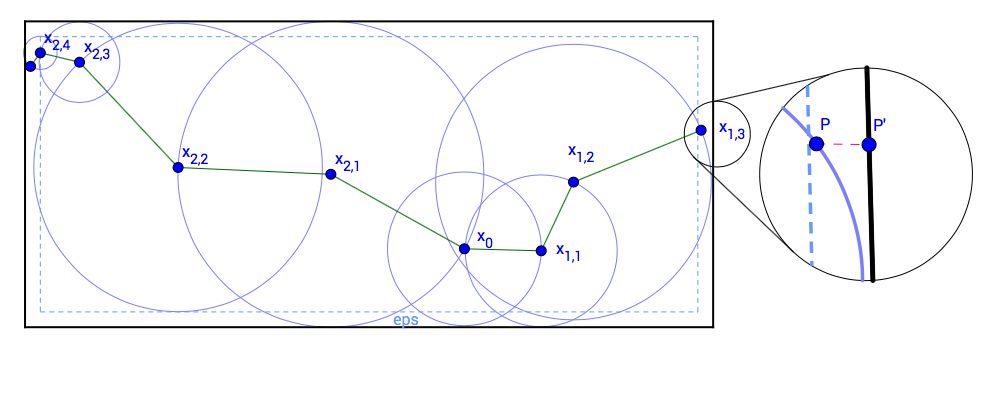
\includegraphics[width=15.0cm]{styles/WoS}
  \caption{2D depiction of \Gls{RWoS}}
\end{figure}

\begin{description}
\item[Origin Point] The origin point describes the discrete point in the domain
$\Omega$ for which a solution to the PDE is to be found. In \ref{diagram}
and in the following passages, this point is also referred to as $x_{0}$.
\item[Radius] The largest distance $r$ from the current point, to the domain boundary
$\partial\Omega$ (depicted above in as lavender circles).
\item[Step] A transition from the current point $x_{i,j}$ to $x_{i,j+1}$ where
$i$ is the path number and $j$ the step number of the current path.  The step has
a length of the radius $r$ and is taken in the uniformly random direction $d$.
\item[Path] The collection of steps from the origin point to the boundary (depicted in green).
\item[Epsilon Boundary] Depicted above as a dotted light blue line, the epsilon boundary
is the allowable deviation from the boundary $\partial\Omega$ a point can display
and still terminate the algorithm (see \ref{sssec:algorithm}).
\item[Projection] Once in the epsilon boundary, a projection of the final point $P$
onto the boundary $\partial\Omega$ is performed, thus creating $P'$.
\item[Evaluation Point] describes $P'$ where the boundary function is evaluated.
The average of the boundary function evaluated at the set of $N$ evaluation points
approximates the solution at the origin point.
\end{description}

\subsection{The Algorithm}\label{sssec:algorithm} %TODO: one or we?
Now that some of the building blocks have been covered, the individual steps of
the algorithm can be discussed.  The goal of the algorithm is to approximate
the solution $u(x_{0})$ at an interior point $x_{0}$ by randomly sampling boundary
values.  This random sampling can be compared to a discrete random integration,
on a sphere around the unknown point, in order to exploit the mean value property
of harmonic functions \ref{sssec:meanvalue}.  Through a recursing execution of this sampling
technique, hopes to reach a known boundary value.
In order to reduce the number of random steps needed to reach the boundary,
one exploits radius independence of $r$ as described in \eqref{eq:radinvar} and takes
the greatest possible $r$ within the domain $\Omega$.  Then a random step direction $d$
is defined by spherical uniform random distribution (for more see \ref{uniformPoints}).
Should one attempt to reach the boundary by this method directly, the probability of the
process terminating can be zero for a substantial subset of domains \cite{kakutani1944, DeLaurentis, Bornemann}.
This is derived from the general case, in which the intersection of the sphere and
the boundary has the probability measure zero. Therefore, one relaxes the
termination condition observes an boundary layer of thickness $\epsilon$ abutting
$\partial \Omega$ in order to ensure termination. This approximation also
serves to reduce the running time of the algorithm (see \ref{epsilonComplexity}). Once in the $\epsilon$
boundary, one projects the current point $P$ onto $\partial \Omega$ ($P'$).  Though this
introduces an error into the approximation, this error can be ensured to be lower than
the sampling error of the Monte Carlo method (see \ref{epsilonDefinition}).  Finally,
$P'$ is evaluated on $\partial \Omega$, concluding the current path, and the process
is repeated.
This algorithm is used to sample $N$ boundary evaluations, the expected value of which,
reflects an increasingly more accurate approximation of the solution $u(x_{0})$
for an ever greater number of trails $N$ \ref{errorAnal} \cite{Bornemann,DeLaurentis}.
  Algorithm \ref{alg:wos} the algorithm presents these steps in pseudo-code.
 \begin{algorithm}[H]{$N, \epsilon, x_{0}$, $\Omega$}
  \caption{Walking On Spheres}
 \label{alg:wos}
\begin{algorithmic}[1]
   \State $sum \gets 0$
  \For{$i\gets1..N$} \label{lst:line:for}
   \State $ r \gets INFINITY$
   \State $x \leftarrow x_{0}$
   \While{$r>eps$}
      \State find largest sphere radius $r$ in $\Omega$ with center $x$ \label{lst:line:radius}
      \State find uniform random direction $d$ on unit sphere \label{lst:line:direction}
      \State $ x \gets x + r\cdot d$ \Comment{update current location}
 \EndWhile
 \State $\overline x \gets project(x)$ \Comment{Project to boundary }
 \State $E \gets f(\overline x)$ \Comment {evaluate boundary value }
 \State $sum \gets sum + E$ \Comment {add result to partial sum} \label{lst:line:reduce}
  \EndFor
 \State $\textbf{return} \text{ } sum / N$ \Comment{return expected value}

\end{algorithmic}
\end{algorithm}

\subsection{Error Analysis}\label{errorAnal}
The algorithmic complexity of \Gls{RWoS} is, of course, an area of interest
when trying to improve performance. Clearly, the larger the number of paths $N$ one
analyzes, the more precise the value estimation.The sampling error (standard deviation)
conforms to the Monte Carlo typical convergence rate and
is $\mathcal{O}(N^{-\frac{1}{2}})$. Furthermore, the estimation error grows proportional to
the boundary layer thickness $\epsilon$.
This error term is due to the projection error at the boundary, and the lost
pseudo Brownian Motion that one ''skips'' via the projection, or  $\mathcal{O}(\epsilon)$.
In total the error amounts to $$Error = \underbrace{ \mathcal{O}(N^{-\frac{1}{2}})}_\text{sampling error} + \underbrace{\mathcal{O}(\epsilon)}_\text{projection error}$$\cite{Bornemann}\label{errorComplexity}.

\subsection{Algorithmic Complexity}

\begin{theorem}
The expected number of steps to reach the $\epsilon$-neighborhood of $\partial\Omega$
is $$\mathcal{O}(\log{}\abs{\epsilon}).$$\cite{Bornemann,DeLaurentis}\label{epsilonComplexity}
\end{theorem}

In light of \ref{epsilonComplexity}, the overall complexity of \Gls{RWoS} can be
defined as $$\mathcal{O}(N \log{}\epsilon)$$ whereby, in our case \ref{epsilonDefinition}
 leads to $$\mathcal{O}(N \log{N^{-\frac{1}{2}}}) = \mathcal{O}(N \log{N}).$$

 This leads to a theoretical dimensionless scalability\cite{Bornemann}.  The practical factuality
 of this claim will be examined later in this work.  %TODO!!!!! and ref!!!

\subsection{Epsilon Selection}

Although Theorem \ref{epsilonComplexity} will be considered as given for this work,
dives deeper into the statistical proof behind this conclusion \cite{DeLaurentis}.  Practically, the
 left path in Figure \ref{diagram} demonstrates the logarithmic convergence a path
 can, and, following \ref{epsilonComplexity} oftentimes does, display via the logarithmic
 nature of the shrinking step size.

 In light of the error analysis depicted in Section \ref{errorComplexity}, it can be observed that the total error is
 determined equally by $\epsilon$ and $N^{-\frac{1}{2}}$. Assuming $ \epsilon \ll N^{-\frac{1}{2}} $ the error term
 is dictated by the sampling size.  Even though the
 smaller choice of $\epsilon$ cannot improve precision, performance is still hurt
 due to the increase in steps per path. Conversely, a large $\epsilon$ would
 restrict the precision to a set level regardless of the number of samples.
 Considering this fact, $\epsilon$ is chosen to allow for
 the greatest possible precision achievable by setting
  $$\epsilon \approx N^{-\frac{1}{2}}$$\label{epsilonDefinition},
 thereby proportionally tying both the error and computational complexity to the
 number of paths $N$ \cite{Bornemann}.
%TODO pi example?
\subsection{Excursion: Uniform Random Directions on a Sphere}\label{uniformPoints}
Given the importance of random directions for \Gls{RWoS}, a brief excursion
into how one can numerically create a uniform distribution on a sphere can prove
to be helpful and insightful.

In order to attain a distribution on a sphere, the process followed herein,
consisted of creating an $n$-dimensional normal distribution in euclidian space and
sampling from the afore-mentioned distribution.  The $n$-dimensional sample vector
is subsequently normalized onto the $n$-dimensional unit sphere.
The 2D case of a uniform
distribution on the unit square being normalized is exemplified below, in order to intuitively
show the distributional discrepancies and obvious ill suited nature for the problem
at hand.  The two point clouds in Figure \ref{plot:distributions} are 2D normal and uniform distributions
respectively.  The peaks on the uniform distribution histogram (Figure \ref{plot:histogram}) stem from the corners
of the distribution in a two dimensional euclidian distribution.  When projected onto
the sphere, the accumulation of points in the corner of the euclidian domain create
''hot spots'' in the spherical distribution.  The two dimensional normal
distribution point cloud (left) on the other hand, mitigates this problem due to the
of the tails of the distributions in the 1D plane, leading to a low probability
in the corners of the square domain.  When the point cloud  is subsequently projected
onto the sphere, it lacks the peaks in the  spherical distribution and displays an
overall uniform nature as can be seen in the relatively constant levels  histogram below (Figure \ref{plot:histogram})
\cite{Yang,Muller1959,marsaglia1972}.

\begin{figure}[htb!]
\begin{center}
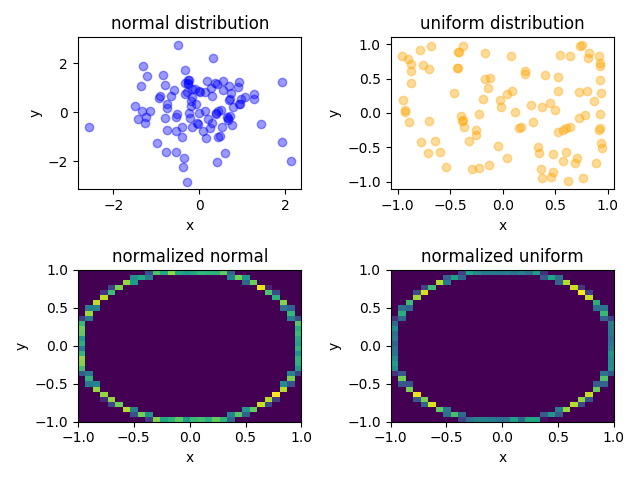
\includegraphics[width=13.5cm]{styles/distributions}
  \caption{}\label{plot:distributions}
  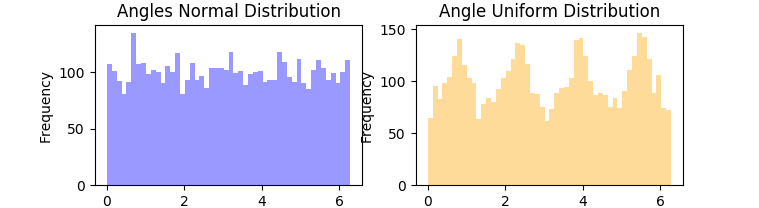
\includegraphics[width=15.0cm]{styles/histograms}
    \caption{}\label{plot:histogram}
\end{center}
\end{figure}
%proof using definitions of sin and cosine similar to the inverse of Tschebychev points


% \subsection{Markov Chains}\label{sssec:markov}
% A Markov Chain is a term used to describe a series of independent events or ''states'',
% who's transition probabilities, i.e. the probability of switching from one state to the
% next, is in independent of past states.  Mathematically this process is described by Howard as:
% \begin{definition}
%   for the set $S$ defined as the finite set of $N$ states, where $s_{i}=\{s_{1},s_{2}\ldots,s_{N}\}\in S$, for simple
%   Markov Processes, the probability of transitioning from state $s_{i}$ to the following state
%   $s_{j}$ is defined by the the probability $p_{ij}$ where $\sum_{j=1}^{N} p_{ij}=1$ and $0 \leq p_{ij} \leq 1$.
%  \cite{howard}\cite{diaconis}.\end{definition}
% In the first pages of his book, Howard graphically depicts this process as,
% \begin{quote}
% ''a frog in a lily pond.  As time goes by the frog jumps from one lily pad to another
% according to his whim of the moment.  The state of the system is the number of the
% pad currently occupied by the frog; the state of the transitions is the course of his leap''
% \cite{howard}\end{quote}
% When the space $S$ is considered to be continuous time, one can speak of a Wiener Process.
%
% %TODO: convergence as in \cite{diaconis}
% \cite{Grindstead}
% \cite{howard}
%
% \subsection{Brownian Motion}\label{sssec:brownian}

% \section{The Random Walks On Spheres Algorithm}
% \Gls{RWoS} is a numerical Monte Carlo Method which employs Brownian Motion
% like random walks to stochastically and discretely solve
% harmonic \glspl{PDE}.
% \par



\subsection{Parallelism}

The intrinsic parallelism in this algorithm is plain to see, namely, one can
exploit the independence of each individual path by executing all paths in parallel
($\mathcal{O}(\frac{N}{w} \log{}N)$ where $w$ is the number of ''worker'' computational units).
This can be realized by unrolling the for-loop in algorithm~\ref{alg:wos}, line~\ref{lst:line:for}.
The resulting intermediate sums $E$ can also be reduced(see: Section \ref{ssec:reduction}) in parallel (algorithm~\ref{alg:wos},
line~\ref{lst:line:reduce}).  Furthermore, for every path step,
the radius and direction are independent (algorithm~\ref{alg:wos}, line~\ref{lst:line:direction} \&~\ref{lst:line:radius}),
 and can therefore be computed in parallel. \cite{Muller,DeLaurentis,Bornemann}
\section{The Basics of Parallel Computing}
In recent years, the convergence towards the physical limits of Moore's law has lead to a
trend towards parallel computing \cite{Kumar}\cite{Markov}.  By most accounts, the
field of Parallel Computing conceived in the early 1958\cite{Gill}, but had previously
been discussed (e.g. Metropolis \cite{Metropolis}). Since then, the field has
 bloomed into the state of the art for high-dimensional simulations and
 other highly parallel applications in
high performance computing as hardware technology has caught up to the first
theoretical speculation of half a century prior. \par

Traditionally, the concept of Parallel Computing was simple: in order to
reduce computation time, one should separate independent steps of a given algorithm
and execute them concurrently upon independent processing units.  In doing so, for a given
problem, which traditionally would have taken time \textit{T}, in the optimal case,
the calculation could be completed in \textit{T/N} time, where \textit{N} describes
the number of processing units being utilized.  This observation was formalized
by Gene Amdahl in 1967\cite{Wilt}:
%
\begin{equation}
  \tag{Amdahl's Law}
  \text{speedup} = S_{latency}(s)= \frac{1}{(r_{s} + \frac{r_{p}}{N})} = \frac{N}{N(1-r_{p})-r_{p}}
  \label{egn:Amdahl}
\end{equation}
%
where \textit{\gls{speed-up}} embodies the factor of temporal acceleration a program
exhibits when additional computational resources are dedicated to its execution.
The variables \textit{$r_{s}$} and \textit{$ r_{p} $} represent the percentage of
 the algorithm that must be executed serially or in parallel, respectively.
   Amdahl's Law describes a computational problem of a fixed dimension,
and the effects of more parallel computing resources on execution time.
This strategy of optimization, in which the size of the problem is constant,
 is called strong scaling.
In the extreme case of unlimited resources, the greatest speed up of a given algorithm
 is limited by it's serial component as we see by taking the limit.
%
\begin{equation}
 \lim_{N\to\infty}  \frac{1}{(r_{s} + \frac{r_{p}}{N})} = \frac{1}{r_{s}} = \frac{1}{1-r_{p}}
\end{equation}
%
This description of optimal \gls{speed-up} does not take into account issues of physical
distance of computing cores or the communication and facilitation overhead between
cores that can occur in real applications, which can lead to lower parallel efficiency.
Nevertheless, the model can serve as a benchmark when analyzing algorithmic
parallelization and the greatest attainable speed-up for a given problem.\par

One further method of quantifying parallelism, is Gustafson's Law\cite{Gustafson}.
%
\begin{equation}
  \tag{Gustofson's Law}
  \text{speedup} = S_{latency}(s) = r_{s} + (1 - r_{p})N
\end{equation}
%
This view of parallelism maintains that `` in practice, the problem
size scales with the number of processes'', and therefore
``assume[s] run time, not problem size, is constant''.
In other words, as the problem size grows, a proportional
amount of resources should be devoted to keep the execution time constant.  This
is called weak scaling.
Both of these laws assist in the quantification of parallel efficiency and
expected gains.

\subsection{Stream Processing and Single Input Multiple Threads}
Stream processing is a paradigm in parallel computing which describes the act
of functions being applied to data in order to compute independent tasks.
The order in which the kernel functions are applied to the data, is determined by
\gls{dd}, which dictate the order and timing of kernel execution. Conventional
sequential computing can be described by a stream process known as \gls{sisd}.
The stream processing paradigm on which GPU programming is based is known as \gls{simt}
 \cite{advancedtopics}.  The idea behind the \gls{simt} paradigm is to over load
 $p$ processors with $t \gg p$ tasks by assigning every processor a \gls{simd} lane
 that executes in lock step.  In adopting this computational paradigm, one can mask
 the computational latency of an individual thread, by switching contexts while
 data dependencies for other tasks are being fetched and
 completing further computations on threads from a separate collection of threads called a warp.  In this way,
 data fetching becomes easier to predict, based on the width of a lane, and more
 data can be processed per \gls{RAM} read.   This masking of latency therefore increases
 the overall throughput of the process \cite{advancedtopics}.


\subsection{GPU Hardware}
When looking to implement efficient numerical code, it is important to understand
 the underlying hardware, in order to exploit architectural intricacies for performance gains.
 To this end, the following passages will be a deep dive into into the history of
 computer architecture and subsequently the design of NVIDA \Glspl{GPU}.
\par
Modern computing architecture was first proposed by John Von Neumann in 1945 \cite{vonNeumann}.
This architecture is composed of three separate sections: the \Gls{CPU}, memory, and \Gls{I/O}.
Modern \Glspl{CPU} are comprised of \Glspl{ALU} which consist of electrical circuits
performing basic mathematical operations, such as addition, subtraction, multiplication and division,
registers, which store the data used for computation by the ALU and cache, which is a more modern development to improve data locality.
\par
By design, \Glspl{CPU} are constructed
to handle general purpose computing workloads.
An \Gls{ALU} completes computational
tasks on an individual datum. By the nature of this
generalized strategy, upcoming computation steps and which data are therefore required,
is unknown to the \Gls{ALU}. If the ALU does not have the data necessary for a computation,
it is forced to wait for the data to be fetched from memory, which can greatly increase computation time.
\par
Transfer times from \Gls{RAM}
are orders of magnitude greater than the computation clock frequency of
a CPU.  This is due to the relatively large physical separation between the CPU and memory,
 the communication overhead needed to fetch the data, and
the nature of \Gls{DRAM}, which electrically refreshes data values at a designated rate.
These problems together are referred to as the Von Neumann Bottleneck\cite{Backus}.
It is important therefore, to develop algorithms and strategies that  predict which data will be required by upcoming operations.
A main focus of modern CPU computation strategies is to always ensure that the data
necessary for a computation is at hand, ready to be used, when requested by the \Gls{ALU}.
The limited number of registers on the ALU meant another, more local storage mechanism
was required.
\par
Cache is a bank of \Gls{SRAM}
that is etched on the same silicon wafer as the CPU itself.  This physical locality,
along with the higher read and write speeds compared to \Gls{DRAM}, lessen the transfer
time of data to the registers, and therefore increase the effective ability of the
 \Gls{ALU} to complete computations. Current caching strategies load data into
 the cache that is either saved near data that is required (data locality based strategy)
 or holds data in the cache that has been used recently (temporal locality strategies).
 The goal of both strategies is to load more data directly from cache, and reduce
 the number of reads and writes from and to \gls{RAM}.
Due to the greater production cost of on-chip cache, its size is limited, and
much research has been dedicated to optimizing cache load strategies of modern CPUs.
\par

It is important to grasp the strengths and weaknesses of modern \Glspl{CPU} to
recognize the computational benefits of \Glspl{GPU}
for modern computations problems.  As the name suggests, \Glspl{GPU} were originally developed
as dedicated computational units for 3D graphics\cite{Sanders}.  They are housed on the same
communication bus as the \Gls{CPU} and memory, and assigned image computational work,
to lessen the load of the \Gls{CPU}.
The GPU is specifically designed to handle workloads on large data sets. Traditionally these
data sets were individual color values for digital images, and the workload as
the transformation of image data to modulate the output on a digital screen.
This heritage defined the strategy modern GPUs take towards computation.
The image data was was relatively high dimensional with intensity values for every pixel in the image.
Each pixel was at least three dimensional (one dimension per color value of red, green and or blue) and
some had a fourth value for alpha transparency. These values would often all undergo
well-defined modulation that could be formulated in a function based on position values.
In the early 2000's these functions were named shaders, and later kernel functions \cite{5751939}.
Due to the independent nature of the execution of kernel functions, the GPUs have multiple, less robust
arithmetic units that perform an individual instruction set on more well defined data.
The well defined execution order leads to less overhead in the execution
model, allowing more resources to be devoted to computation.
The dimensionality of the data being computed leads to \Glspl{GPU} having larger registers \cite{5751939},
which allow for fewer context switches, and therefore greater \gls{ai}.  Overall
Through put is valued more than single thread execution speed.  %lower thermal density?

\subsection{GPU Architecture}\label{ssec:gpu_architecture}
The GPU hardware architecture and terminology of said architecture varies from
vendor to vendor.  For the sake of uniformity, this document will adopt the
terminology employed by the manufacturer, NVIDIA.  To begin, in the following passages the CPU
will occasionally be referred to as the \textbf{host} while the GPU will be referenced as \textbf{device}.
These are standard terminologies in GPU programing. GPUs are comprised of four major components:
\begin{description}
  \item[Host interface] moderates communications between the host and the device.
  Commands are dispatched to the necessary hardware, and synchronization between
  host and device is managed through this interface.
  \item[Copy Engine] manages the bidirectional transfer of data between the host
  and device.  Modern hardware can have 0-2 Copy Engines per device in order to
  manage the conversion of linear memory to CUDA arrays while saturating the PCI
  bus.  The independence of the Copy Engine(s) allows for concurrent data transfers
  and computation.
  \item[DRAM Interface] a memory interface with a bandwidth of up to 100Gb/sec\cite{Wilt}.
  Some interfaces also support device side L2 caches usage.
  \item[TPCs \& GPCs] \underline{T}exture \underline{P}rocessing \underline{C}luster
  and \underline{G}raphics \underline{P}rocessing \underline{C}lusters are an assembly
  of \Glspl{SM} along with cache for computation.
  \item[\Glspl{SM}] a collection of \Glspl{ALU} or ''CUDA cores''
\end{description}\cite{Wilt}

\subsubsection{Streaming Multiprocessors}
Each GPC contains a cluster of SM's.  The number of SM's per cluster varies by
model of GPU. SM's are comprised of a collection of CUDA-cores.  Some examples
 can be found in table below.
\begin{table}[htb!]
\caption{"collection of NVIDIA \Glspl{GPU} technical specifications"}
\begin{center}\label{hardwareTable}
\begin{tabu} to 0.9\textwidth { | X[l] | X[c] | X[c] | X[c]| X[c]| X[c]| X[r] | }

 \hline
 Model & GPU Architecture &Frequency& Single-Precision Performance & CUDA-Cores & CUDA-Cores per SM & GPU Memory \\
 \hline
 Tesla P100 & NVIDIA Pascal &1328 MHz &9.3 TFLOPS & 3584 & 64 & 16GB at 732.0 GB/s\\
 \hline
 GTX Titan X & NVIDIA Pascal & 1000 MHz & 11 TFLOPS & 3584 & 64 & 12GB at 336.5 GB/s\\
 \hline
 GTX 560 Ti & NVIDIA Fermi & 822 MHz&12634 GFLOPS & 384 & 32  & 1GB at 128.27 GB/s\\
\hline
\end{tabu}
\end{center}
\end{table}

Each SM is comprised of
\begin{itemize}
  \item execution units for 32-bit integer, as well as single and double precision arithmetic,
  \item special function units for log/exp sin/cos and sqrt functions,
  \item a warp scheduler to coordinate the dispatch of threads,
  \item a constant cache to broadcast data to SM's,
  \item shared memory accessible by all threads,
  \item and texture mapping hardware %\cite{Wilt}.
\end{itemize}

This basic overview of the architecture of the hardware is important to understand
how the the programming API maps to the available hardware.


\section{Parallel Computing with CUDA}
\subsection{CUDA Software}

The CUDA parallel computing environment is a C++ language wrapper with built in
\gls{directive pragmas} to interact with the NVIDIA hardware.  Although CUDA is modeled on the
hardware it runs on, it is not wholly analogous with the hardware architecture,
and higher level concepts have been added to aid in the usage of CUDA code.
\par
The CUDA ecosystem stack is comprised of five layers accessible to the user.
These layers are the CUDA application itself, CUDA Libraries, CURA Runtime otherwise
known as CUDART, and the CUDA Driver.


\subsubsection{CUDA Libraries}

The highest level of this stack is occupied
by CUDA libraries. When looking to optimize code with CUDA, a
first step should be to take advantage of CUDA Libraries.  These highly optimized
and user friendly libraries, such as CUBLAS and CUDA Thrust, allow the use of
CUDA hardware, with minimal understanding of the underlying hardware or execution strategy.
They can prove to be indispensable tools for beginner users or those looking to quickly and
efficiently prototype a problem in C++. The author recommends their use as the first step
in any CUDA based undertaking. They provide the ability to create a quick proof
of concept for a project, as well as a highly optimized base line, should further
development be planned.
\subsubsection{CUDA Runtime}

Moving down the stack, CUDA runtime provides an interface to the user, which mirrors
standard C functionality such as malloc and memcpy.  These functions differentiate
themselves from host functions with the prefix \textit{``cuda''} or \textit{``cu''}
e.g. \incpp{cudaMalloc()} and \incpp{cudaMemcpy()}.  Functions that are to be executed on the
device, are called kernels or kernel functions, which can be identified
 via their triple angle bracket syntax, ``$<<< >>>$''.
Kernel parameters can be specified in these triple angle brackets.  These parameters
include number of blocks per grid, threads per blocks, size of shared memory and
stream, all topics which shall be discussed later in this document (\ref{btg}).

\subsubsection{CUDA Driver API}
The CUDA driver is the interface to lower lever command sets used by the CUDA driver, which allows more detailed control
of kernel calls and memory allocation. Many of the same functionalities are possible,
but execution is more tedious and requires a large number of individual commands
when carrying out operations \cite{driver}. This granularity of control can nevertheless be
helpful when tuning a program and striving for higher execution performance.
\subsubsection{CUDA Driver}

The CUDA driver is the lowest level of integration between the host and the device
and facilitates communication between the \Gls{GPU} and the rest of the computer via the bus.


\subsection{Compilation and Execution}


CUDA programs are written in CUDA flavor C++.  The CUDA flavored of C++
can be compiled via a compiler driver tool called nvcc, which can compile, link and execute CUDA code.  This process occurs
 in three main steps.
 \begin{enumerate}

\item First,
files containing CUDA pragmas are assigned the .cu ending format, and split upon
compilation into device and host sections.
\item Second, these files are subsequently
compiled separately into to host and device machine code respectively.
\item Lastly, both compilates are merged into a single executable, to be run on the host.
\end{enumerate}
\par
Device machine code, is referred to as \hyphenation{mi-cro-code} \textit{microcode},
which is compiled for a specific device model's architecture. In order to be able
to execute the same executable
on multiple \Glspl{GPU} and to allow backwards compatibility of CUDA features, CUDA code is
first compiled into \Gls{PTX}, a pseudo-assembly language.  \Gls{PTX} is then
further compiled in to device microcode and written into a CUDA binary file called .cubin.
This can either happen offline, at compile time,
or online, at runtime, in a \gls{jit} fashion.  By default, both
the microcode for the local device present at compilation and the generalized
\gls{PTX} compilates are added to the to the executable file.
This way, should the executable be run on a different device, the \gls{PTX} can
be recompiled appropriately with \Gls{jit} compilation, and executed on the a
desired device\cite{Wilt}.

\subsection{Programming CUDA}

There are many parallel contexts when programming CUDA. To help developers conquer
the challenges of parallel programming, CUDA offers a multi-contexts development
environment to help break problems down into sub-problems, that can be then translated
by the compiler into parallel code. The following explanation, is only meant to
give the reader insight into the CUDA syntax, thereby allowing comprehension of
the subsequent work. For a more complete and elaborate explanation of CUDA, other
more extensive resources are recommended \cite[etc.]{Wilt,Sanders,driver}.
%separate address space from CPU --> mem copies
%blocks and threads
\subsubsection{Blocks, Threads and Grids}\label{btg}
%TODO: insert diagram of threads blocks and grids
The two main contexts of parallelism in CUDA are CUDA blocks and CUDA threads.
Threads can be thought of as a sequence of operation commands for an individual registers, with an assortment of computational
functionality.  Threads should are completely independent from one another,
and only synchronized through explicit call to synchronization functions called via the \textit{\_\_syncthreads()} command. Threads, like
registers, can only work on one datum at a time, but are all executed simultaneously.
Threads are, in turn, organized into blocks, and a collection of blocks comprises a grid.
Blocks are an abstraction of a process on an SM.  If a block is smaller than
the computational capacity of an SM, then tasks from multiple blocks can be computed
simultaneously.  This is referred to as block occupancy.  If resources allow, multiple blocks can
be executed on an \Gls{SM} simultaneously. Since neither the number of blocks nor the
number of threads are limited by the limited by the number of registers and \Glspl{SM},
but rather can exceed hardware values, the analogy stops here.  Both
threads and blocks can be described by an abstraction of a hardware feature, although one should try to
consider hardware contexts and software separately from one another, as to reduce the number
of false assumptions.
\par
For ease of programming, the current thread or block ID can be retrieved using
 \incpp{threadIdx.{x,y,z}} and \incpp{BlockIdx.{x,y,z}}. As can be deduced via the nomenclature,
 these variables are multi-dimensional, a feature that can be advantageous in some
 applications such as computer vision, but is not a necessity in other applications
where the problem does not map to a 2D or 3D euclidian space. Further variables,
for the dimension of the grid and block are also available. %TODO: Create table as on page 213
The number of threads and blocks assigned to a problem is relatively arbitrary and can
be designated by the developer before hand, or dynamically.  There are however limits
to this flexibly that are described in the CUDA documentation\cite{bestpractices}.
  Also, minor performance
repercussions could be experienced, if the dimensionality of the framework is poorly
chosen.
%kernel syntax
\subsubsection{Kernels}

At the core of any CUDA program, is the kernel. Kernels make up the basic instruction
set that one often finds in any other serial program as well, the only difference being,
where as in a serial program one would iterate over data by means of a loop,
CUDA kernels are executed on every data in an array in an \gls{simt} fashion.

%TODO: vector addition example

The angle brackets in front of the kernel call identify the function as a kernel,
and allow syntax  identification during compilation of a program.  Depending on
whether a device kernel is to be called from the host or internally from the device,
kernels can be labeled with the pragma \incpp{__global__} or \incpp{__device__}  respectively.
Kernels declared \incpp{__global__} can be called from both the host and device, while \incpp{__device__}
kernels are only available from the device.
The identifier \incpp{__host__} allow for kernels to be called from and run on the host.

The parameters in the triple angle brackets are, from left to right, grid size or number of blocks,
block size or number of threads, size of shared memory, and stream ID.  While grid and block size,
are required values, the size of shared memory can also be statically allocated from within
a kernel (more on shared memory in \ref{sssec:memories}).  Dynamic allocation though requires the kernel to be called parameterized with
the size, and the value to be initialization from within the kernel function.  The stream
parameter also is set to main stream by default, but must be set by the user when
working with multiple streams (more on streams in: \ref{sssec:streams}).
%shared vs. global memory
\subsubsection{Memories}\label{sssec:memories}
GPU memory does not benefit from features such as virtual
memory or paging, as one might expect from CPU memory. Instead, devices have an
address space completely separate from the host address space, where every address is assigned a physical space in memory.
In many cases, memory consists of a dedicated chip on the device that is controlled
by the memory controller.  This memory must be managed by the user when programming in CUDA.
\par
Not all device memories are created equal.  Similarly to \Glspl{CPU},
different memories have varying strengths and weaknesses.  By preallocating memory for a variable,
that is either read only, or read and written often, one can greatly increase the
performance of ones program\cite{Wilt}.   %TODO: CUDA attempts to avoid lazy allocation--> performance gains.
There are four main types of CUDA memories.
\begin{description}
  \item [Global memory] Memory on the Device with bandwidth of up to 100 Gb/sec.
  Global memory is allocated dynamically by the user via cudaMalloc() and cudaFree() functions.
  Dynamic allocation is normally performed in host code, due to large performance shortfall
  when implemented in a kernel call.
  \item [Constant memory] optimizes for read only memory on device for higher
  read speeds.  The constant declaration is beneficial for broadcast style data
  reads, in other words, when every thread is to receive the same data.
  \item [Texture memory] Constant declaration of global memory with dedicated
   texture access pattern controller.  Texture memory allows performance benefits
   for uncoelessed variable access, which would normal lead to large performance
   degradation with normal global memory.
  \item [Shared memory] User managed cache located on every \Gls{SM}.  Shared memory access
  normally benefits from a 10x speed increase over global memory access, while it remains
  10x slower than register reads \cite{Wilt}.  These performance gains are dependent
  on the shared memory read strategy.  In oder to avoid block conflicts, and therefore
  performance degradation, thread based coalesced memory reads and writes are to
  be strived for.
  \item [Local memory] local memory contains the program stack for every thread
  in a CUDA program. Should a program run out of registers for thread local variables,
  local memory is  used to store overflow variables. This variable overflow is often
  linked to detrimental performance losses and should be avoided \cite{Wilt}.
  \item [Cache] Similarly to CPU's Cache is also realized on GPU \glspl{SM} in order
  to reduce transfer latency.  \glspl{GPU} however employ a different caching strategy,
  due to the \gls{simt} computational approach.
  \item [registers] Memory units on \Gls{SM} used to store thread local variables,
                    and variables for current computation.
\end{description}

%streams
\subsubsection{Streams}\label{sssec:streams}
CUDA Streams enable the coarsest level of concurrency in the CUDA API.  Streams
 consist of a series of commands that are to run in series.  Commands assigned
a different set of streams can be executed in parallel. Memory transfers and
kernels can be assigned separate streams in order to create a workflow pipeline and increase
the overlap between data transfers and data computation. This is made possible by the
independent Copy engine as mentioned in \ref{ssec:gpu_architecture}.  Furthermore,
on systems with more than one \Gls{GPU}, streams can allow both data transfers and
kernels to be excited concurrently on separate \Glspl{GPU}, leading to even greater
performance.
